\documentclass[aspectratio=169]{beamer}

\usetheme{default}
\setbeamertemplate{navigation symbols}{}
\setbeamertemplate{itemize item}{\color{black}\textbullet}
\setbeamertemplate{itemize subitem}{\color{black}\textbullet}
\usepackage{xcolor}
\definecolor{navy}{RGB}{0, 0, 128}
\definecolor{lightblue}{RGB}{230,240,250}
\definecolor{darkgreen}{RGB}{0,100,0}
\definecolor{lightgreen}{RGB}{230,250,230}
\newcommand{\highlight}[1]{\colorbox{lightblue}{$\displaystyle\textcolor{navy}{#1}$}}
\newcommand{\highlighttext}[1]{\colorbox{lightblue}{\textcolor{navy}{#1}}}
\newcommand{\highlightgreen}[1]{\colorbox{lightgreen}{$\displaystyle\textcolor{darkgreen}{#1}$}}

\begin{document}

\begin{frame}
\centering
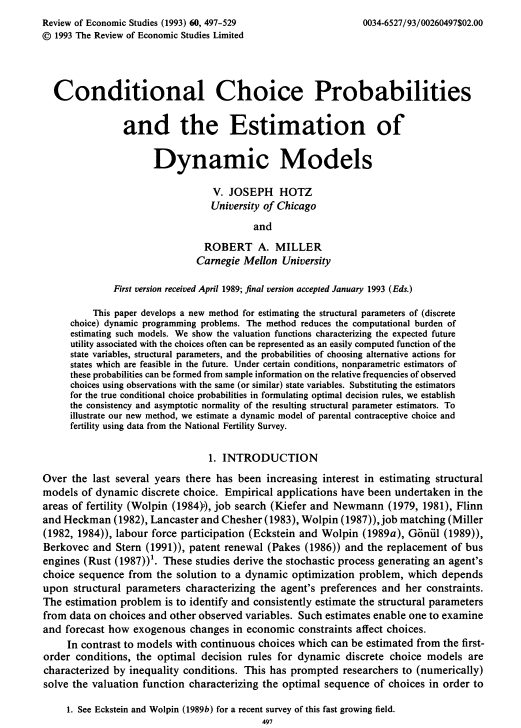
\includegraphics[width=.42\textwidth]{HotzMiller_cover.jpg}
\end{frame}


\begin{frame}

\onslide<1->{
Key insight: Differenced $v_j - v_{j'}$ can be mapped into CCPs ($p_j$'s)
}

\bigskip{}

\onslide<2->{
Method: Extract $p_j$'s from data in first stage, avoid solving backwards recursion
}

\bigskip{}

\onslide<3->{
Application: Couples' fertility decisions (optimal stopping problem)
}

\end{frame}




\begin{frame}

Consider an individual with two choices and Type 1 Extreme Value errors

\bigskip{}

\onslide<2->{
Probability of choice 1:
\begin{align*}
p_1 &= \frac{\exp(v_1)}{\exp(v_0) + \exp(v_1)}
\end{align*}
}

\onslide<3->{
Ratio of probabilities:
\begin{align*}
\frac{p_1}{p_0} &= \frac{\exp(v_1)}{\exp(v_0)} = \exp(v_1 - v_0)
\end{align*}
}

\onslide<4->{
Taking logs:
\begin{align*}
\log\left(\frac{p_1}{p_0}\right) = \log\left(p_1\right) - \log\left(p_0\right)  &= v_1 - v_0
\end{align*}
}

\onslide<5->{
Works for any two alternatives!
}

\end{frame}




\begin{frame}
Let's look at it equivalently from the standpoint of $V_{t+1}$, assuming $\epsilon$'s are T1EV:
\bigskip\par
\only<2>{
\begin{align*}
V_{t+1} &= \mathbb{E}\max_{j \in \mathcal{J}}\left\{v_{jt+1}+\epsilon_{jt+1}\right\}\\
&\\
&\phantom{=\log\left(\sum_k \exp\left(v_{kt+1}\right)\right)}
\end{align*}
}
\only<3->{
\begin{align*}
V_{t+1} &= \mathbb{E}\max_{j \in \mathcal{J}}\left\{v_{jt+1}+\epsilon_{jt+1}\right\}\\
&\\
&=\log\left(\sum_k \exp\left(v_{kt+1}\right)\right) + c
\end{align*}
}

\onslide<4->{
\bigskip\par
Can do some algebra to show that $V_{t+1} = v_{jt+1} - \log \left(p_{jt+1}\right) + c$ for any alternative $j$
}

\end{frame}




\begin{frame}

Key derivation trick: multiply and divide inside the log sum by $\exp(v_j)$

\bigskip{}

\only<1>{
\begin{align*}
V_{t+1} &= \log\left(\sum_k\exp(v_{kt+1})\right) + c
\end{align*}
}

\only<2>{
\begin{align*}
V_{t+1} &= \log\left(\frac{\exp(v_{jt+1})}{\exp(v_{jt+1})}\sum_k\exp(v_{kt+1})\right) + c
\end{align*}
}

\only<3>{
\begin{align*}
V_{t+1} &= \log\left(\exp(v_{jt+1}) \cdot \frac{\sum_k\exp(v_{kt+1})}{\exp(v_{jt+1})}\right) + c
\end{align*}
}

\only<4>{
\begin{align*}
V_{t+1} &= \underbrace{\log\exp(v_{jt+1})}_{v_{jt+1}} + \log\left(\underbrace{\frac{\sum_k\exp(v_{kt+1})}{\exp(v_{jt+1})}}_{\left(\frac{1}{p_{jt+1}}\right)}\right) + c
\end{align*}
}

\only<5>{
\begin{align*}
V_{t+1} &= v_{jt+1} + \log\left(\frac{1}{p_{jt+1}}\right) + c
\end{align*}
}

\only<6->{
\begin{align*}
V_{t+1} &= v_{jt+1} - \log \left(p_{jt+1}\right) + c \quad\quad \forall\, j \in \mathcal{J}
\end{align*}
}

\end{frame}


\begin{frame}

\onslide<1->{
For T1EV, we showed earlier:
$$v_j - v_0 = \log(p_j) - \log(p_0)$$
}

\onslide<2->{
Define the mapping:
$$\psi_0^j(p) = \log(p_j) - \log(p_0)$$
}

\onslide<3->{
\bigskip\par
This is our \textcolor{navy}{inversion formula} for the logit case
\bigskip\par
}

\begin{itemize}
\itemsep1.5em
    \item<4-> \textcolor{navy}{Regular (no $\psi$)}: solve for $v_j-v_0$ $\to$ compute $p_j$ $\to$ estimate parameters
    \item<5-> \textcolor{navy}{Inversion (using $\psi$)}: observe $p_j$ $\to$ recover $v_j-v_0$ $\to$ estimate parameters
\end{itemize}
\end{frame}



\begin{frame}

Hotz-Miller inversion proposition: 
\bigskip\par

There exists an invertible mapping $\psi$ from CCPs ($p$'s) to $(v_j - v_k)$'s
\bigskip\par

For sake of example, let's consider $j=0$

\begin{align*}
\onslide<2->{V_{t+1} &= \mathbb{E}\max\{v_{0t+1} + \epsilon_{0t+1}, v_{1t+1} + \epsilon_{1t+1}, \ldots, v_{Jt+1} + \epsilon_{Jt+1}\}\\[1.5em]}
\only<3>{&= \highlight{v_{0t+1}} + \mathbb{E}\max\{\epsilon_{0t+1}, \highlight{v_{1t+1} - v_{0t+1}} + \epsilon_{1t+1}, \ldots, \highlight{v_{Jt+1} - v_{0t+1}} + \epsilon_{Jt+1}\}\\[1.5em]}
\only<4,5>{&= v_{0t+1} + \mathbb{E}\max\{\epsilon_{0t+1}, v_{1t+1} - v_{0t+1} + \epsilon_{1t+1}, \ldots, v_{Jt+1} - v_{0t+1} + \epsilon_{Jt+1}\}\\[1.5em]}
\only<5>{&= v_{0t+1} + \mathbb{E}\max\{\epsilon_{0t+1}, \psi_0^1(p_{t+1}) + \epsilon_{1t+1}, \ldots, \psi_0^J(p_{t+1}) + \epsilon_{Jt+1}\}}
\only<6->{&= v_{0t+1} + \mathbb{E}\max\{\epsilon_{0t+1}, \highlight{v_{1t+1} - v_{0t+1}} + \epsilon_{1t+1}, \ldots, \highlightgreen{v_{Jt+1} - v_{0t+1}} + \epsilon_{Jt+1}\}\\[1.5em]}
\only<6->{&= v_{0t+1} + \mathbb{E}\max\{\epsilon_{0t+1}, \highlight{\psi_0^1(p_{t+1})} + \epsilon_{1t+1}, \ldots, \highlightgreen{\psi_0^J(p_{t+1})} + \epsilon_{Jt+1}\}}
\end{align*}

\onslide<7->{
\bigskip\par
This mapping $\psi\left(\cdot\right)$ works for \textit{any} distribution of $\epsilon$!
}

\end{frame}




\end{document}